\section{Results} 
\label{sec:results}
%\vspace{-2ex}
Fig~\ref{fig:appTable} lists all the benchmarks which have been successfully evaluated with SecondWrite prototype. It includes the complete SPEC2006 benchmark suite, benchmarks from other suite and a real world program, Apache server. As evident from Fig~\ref{fig:appTable}, SecondWrite is able to correctly handle binaries from three different programming languages (C, C++, Fortran), two different compilers (gcc and Visual studio) and two different OS (Linux and Windows), demonstrating the robustness of our techniques. Benchmarks on Linux are compiled with gcc v4.4.1 (O0 (No optimization) and O3 (Full optimization) flags) without any symbolic or debug information. Results are obtained for \emph{ref} datasets
on a 2.4GHz 8-core Intel Nehalem machine running Ubuntu. Windows benchmarks are compiled with Microsoft Visual Studio compiler (O0 (No optimization) and O2 (Maximum optimization) flags). \emph{Only the C and C++ programs are included for Windows since VisualStudio does not compile Fortran}. In the case of Apache server, we tested a \emph{http} server with the rewritten binary. Apache server, being an interactive program, is not amenable to performance analysis like other benchmarks; hence we only provide its static results.
%It is a diverse set of programs totalling more than 400K lines of code. 
%We were also able to correctly apply the standard suite of LLVM transformation passes without any changes.  
%A subset of \emph{SPEC} benchmarks, \emph{OpenMP} benchmarks and a few real world programs are evaluated to substantiate the performance of our rewriter. 
\begin{figure}[t]
{
%\vspace{-0.2in}
\centering
%\psfig{figure=figures/plots/runtimeFinal.eps,width=5.5in} }
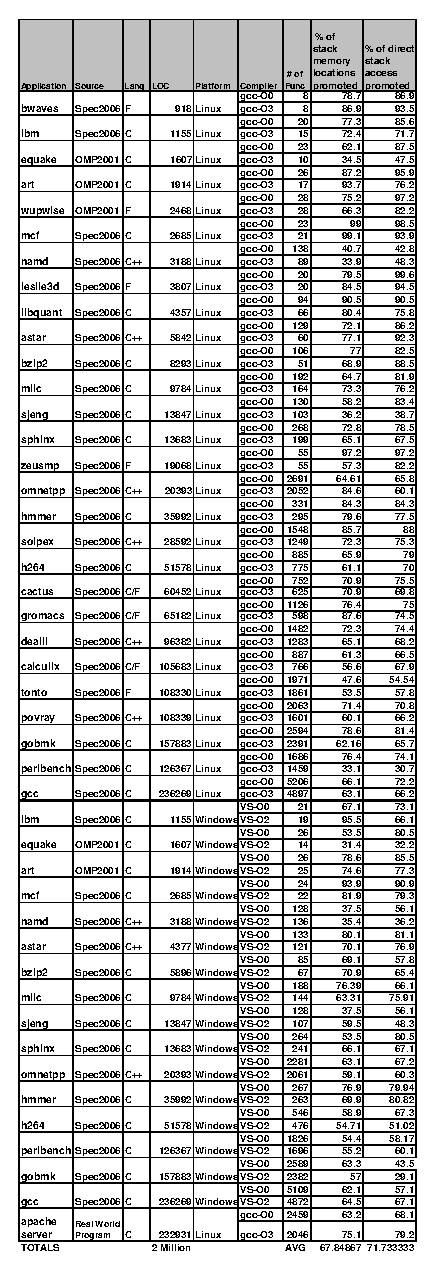
\includegraphics [width=0.7\linewidth] {figures/EPS/appTablenew2.eps} 
%\vspace{-3ex}
\caption { \textit{Benchmarks Table}}
\label{fig:appTable}
}
\vspace{-2ex}
\end{figure}
 

%%\begin{figure}[t]
%\vspace{-0.5in}
%\centering
%\psfig{figure=figures/plots/runtimeFinal.eps,width=5.5in} }
%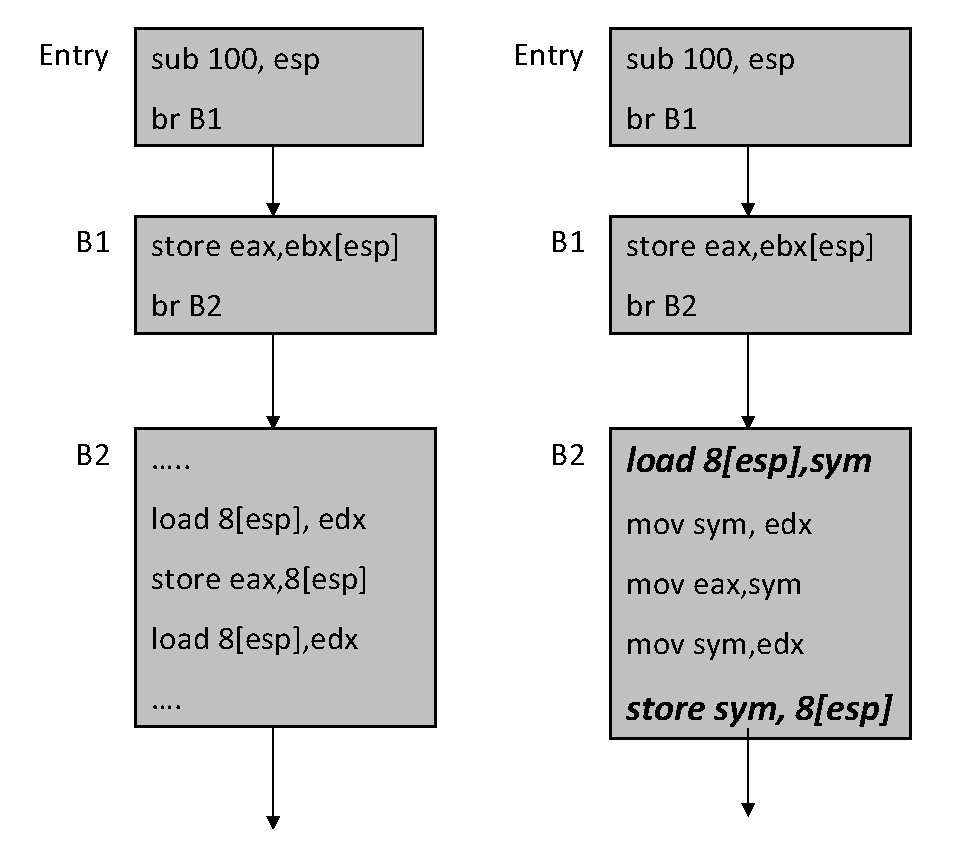
\includegraphics [width=0.5\linewidth] {figures/EPS/cfgex.eps} 
%\tiny{
%\caption { \textit{Stack layout in a binary}}
%}
%\label{fig:stack-layout}
%\end{figure}

\begin{figure}[b]
{
\vspace{-2ex}
\centering
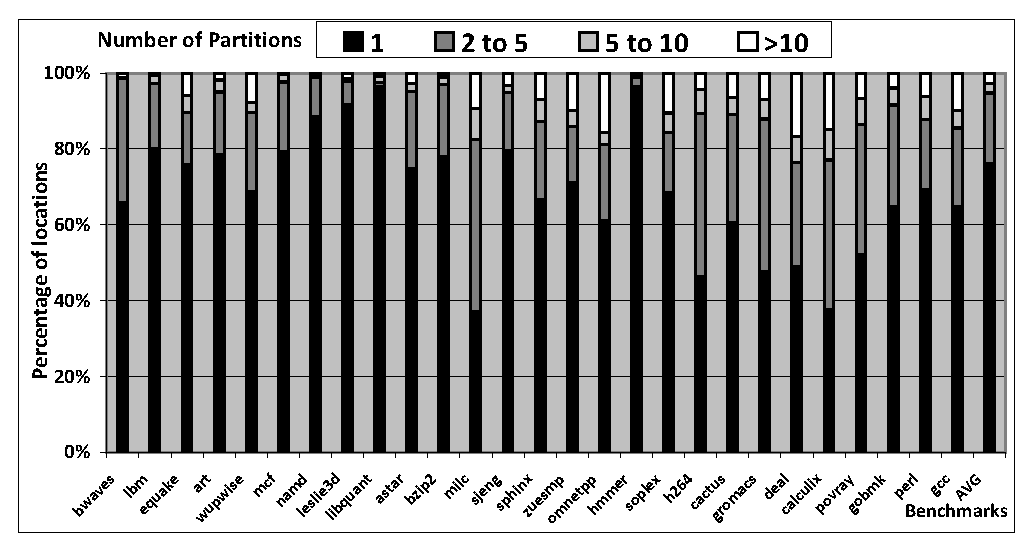
\includegraphics[width=0.8\linewidth]{figures/EPS/partition-visualization-2.eps}
%\vspace{-3ex}
\caption{\textit{Partition algorithm visualization }}
\label{fig:PartResult}
}
%\hfill
\vspace{-3ex}
\end{figure}




%\begin{figure}[t]
%{
%\centering
%\begin{minipage}{.6\linewidth}
%{
%\centering
%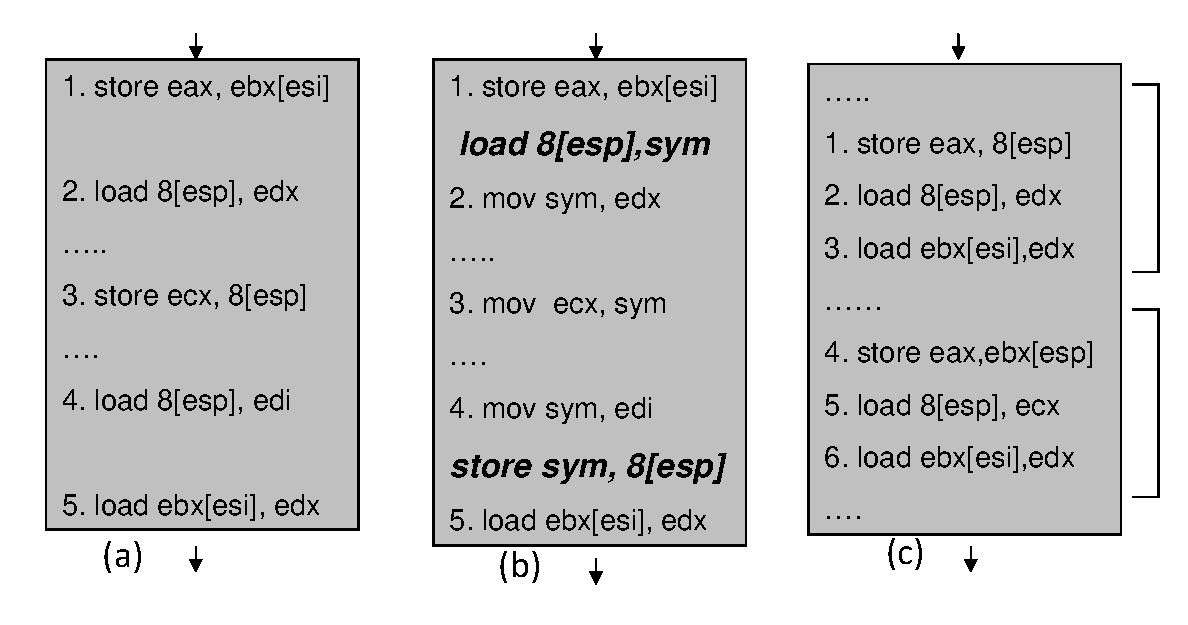
\includegraphics[width=0.5\linewidth]{figures/EPS/pathcfg.eps}
%\caption{\textit{Path dependent promotion. Second operand in the instruction is the destination of the instruction. }}
%\label{fig:PromExample}
%}
%\vspace{-0.1in}
%\end{minipage}
%%\hfill
%\begin{minipage}{0.3\linewidth}
%{
%\centering
%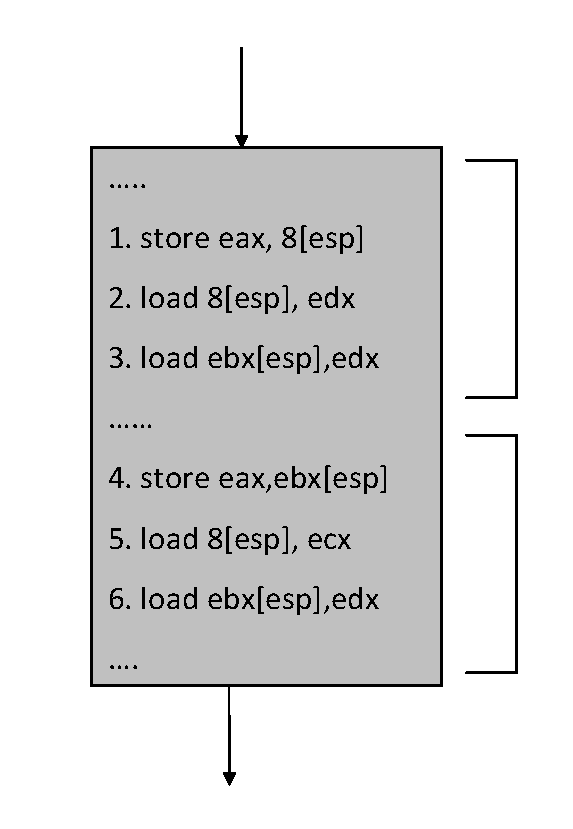
\includegraphics[width=0.3\linewidth]{figures/EPS/partitioncfg.eps} 
%\caption{\textit{Motivation for partition}}
%\label{fig:PartExample}
%}
%\vspace{-0.1in}
%\end{minipage}
%}
%\vspace{-0.2in}
%\end{figure}

\subsection{Static characteristics}
Fig~\ref{fig:appTable} displays the static characteristics of symbol promotion techniques - the percentage of stack memory locations promoted to symbols and the percentage of direct stack memory accesses promoted to symbol accesses in the IR and in the recovered source-code. The results depict that on average, 67\% of stack locations are promoted to symbols resulting in promotion of 72\% of direct stack accesses. For the remaining memory operations, the net benefit for promotion didn't meet the corresponding threshold. Theoretically, our framework can achieve \emph{100\% symbol promotion} if the promotion threshold is ignored, but this leads to high overhead in the rewritten binaries due to \emph{Promoting Loads} and \emph{Promoting Stores}. The development of more advanced alias analysis would improve results of our symbol promotion without adversely affecting the performance.

\begin{figure*}[t]
{
\vspace{-0.3in}
\begin{minipage}{.32\linewidth}
\centering
{
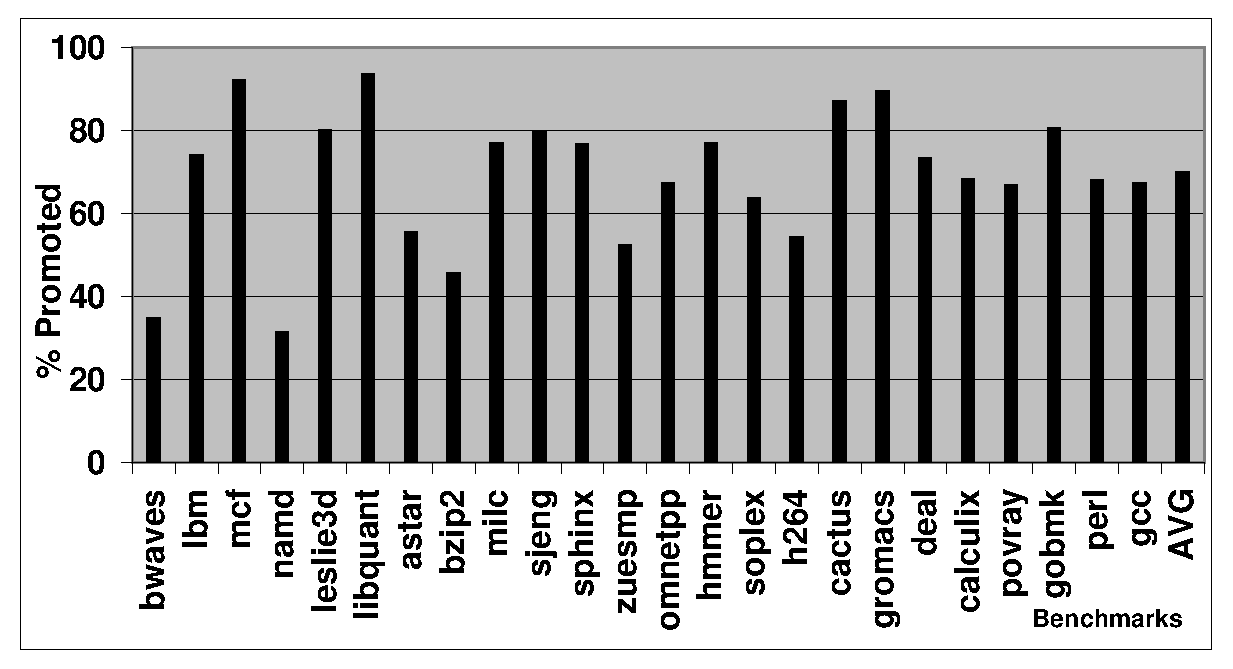
\includegraphics[width=\linewidth]{figures/EPS/origSymPromotion.eps}
\caption{\textit{Percentage of original symbolic accesses recovered in IR}}
\label{fig:OrigSymPromResult}
}
\end{minipage}
\hfill
\begin{minipage}{.38\linewidth}
\centering
{
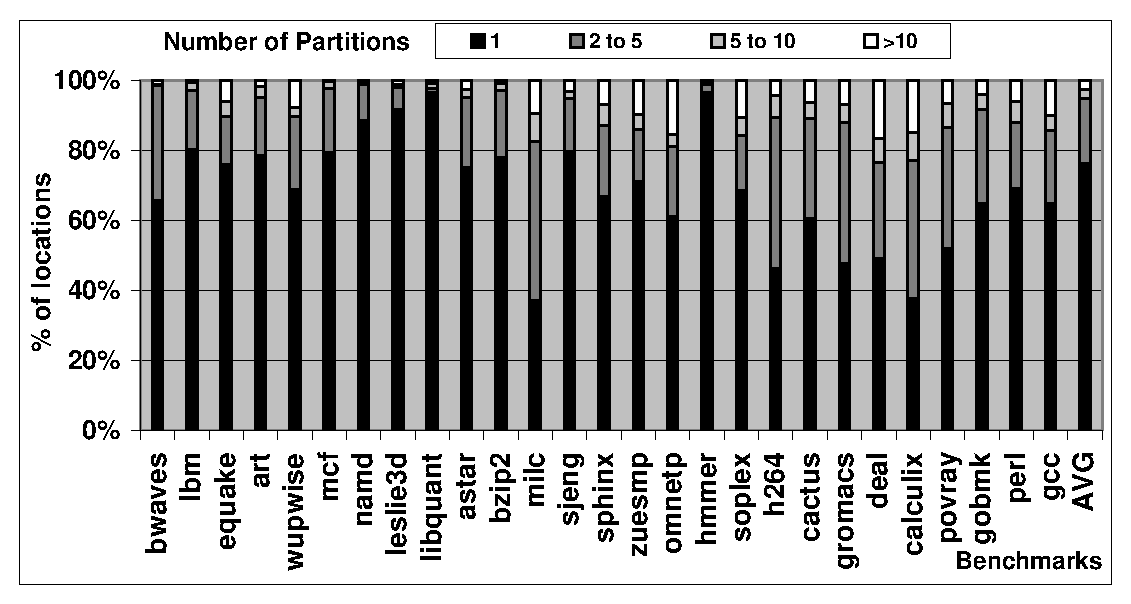
\includegraphics[width=\linewidth]{figures/EPS/partition-visualization.eps}
\caption{\textit{Partition algorithm visualization}}
\label{fig:PartResult}
}
\end{minipage}
\hfill
\begin{minipage}{.29\linewidth}
\centering
{
\begin{tiny}
\begin{tabular}{|c|c|c|c|} %|r|r|r|}
%xxxxx\=xxxxxxxxxxxxx\=xxxxxx\=xxxxxxxxxxx\=xxxxxx\=  \kill\\
\hline
\textbf{Program}&{\textbf{Version}}&{\textbf{Physical stack}}&{\textbf{Run Time}}\\
{}&{}&{}&{\textbf{Checks}}\\ \hline
gcc&gcc-O0,VS-O0&117&0\\\hline
gcc&gcc-O3, VS-Ox&117&10\\	\hline
tonto&gcc-O0, gccO3&20&0\\	\hline
\end{tabular}
\caption {{\textit{Programs demonstrating corner cases of our analysis }}}
\label{fig:resultsCornerCases}
\end{tiny}
%\vspace{-4ex}
}
\end{minipage}
}
\vspace{-3ex}
\end{figure*}
\begin{figure*}[t]
{
%\vspace{-1.2in}
\begin{scriptsize}
%\centering
\begin{minipage}{.35\linewidth}
\centering
{
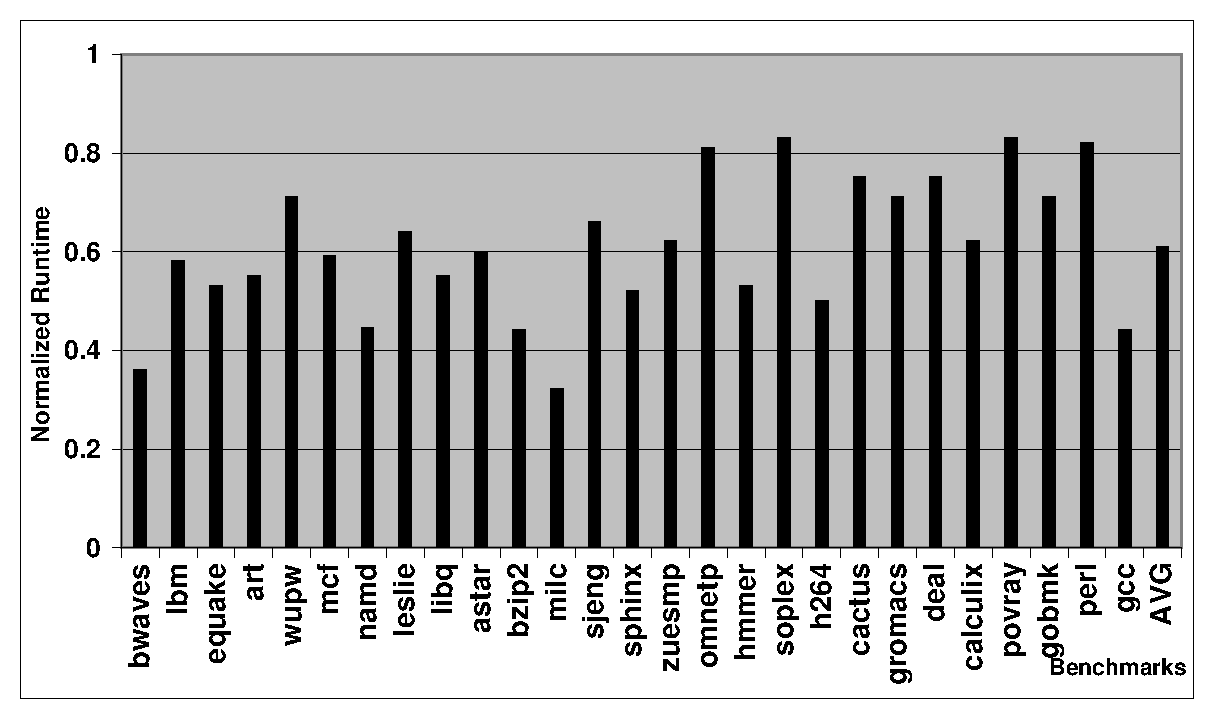
\includegraphics[width=\linewidth]{figures/EPS/unoptperf.eps}
\begin{scriptsize}
\caption{{ {\textit{Normalized runtime of rewritten binary as compared to unoptimized gcc input binary (=1.0)}}}}
\label{fig:unoptimized}
\end{scriptsize}
}
\end{minipage}
\hfill
\begin{minipage}{.35\linewidth}
\centering
{
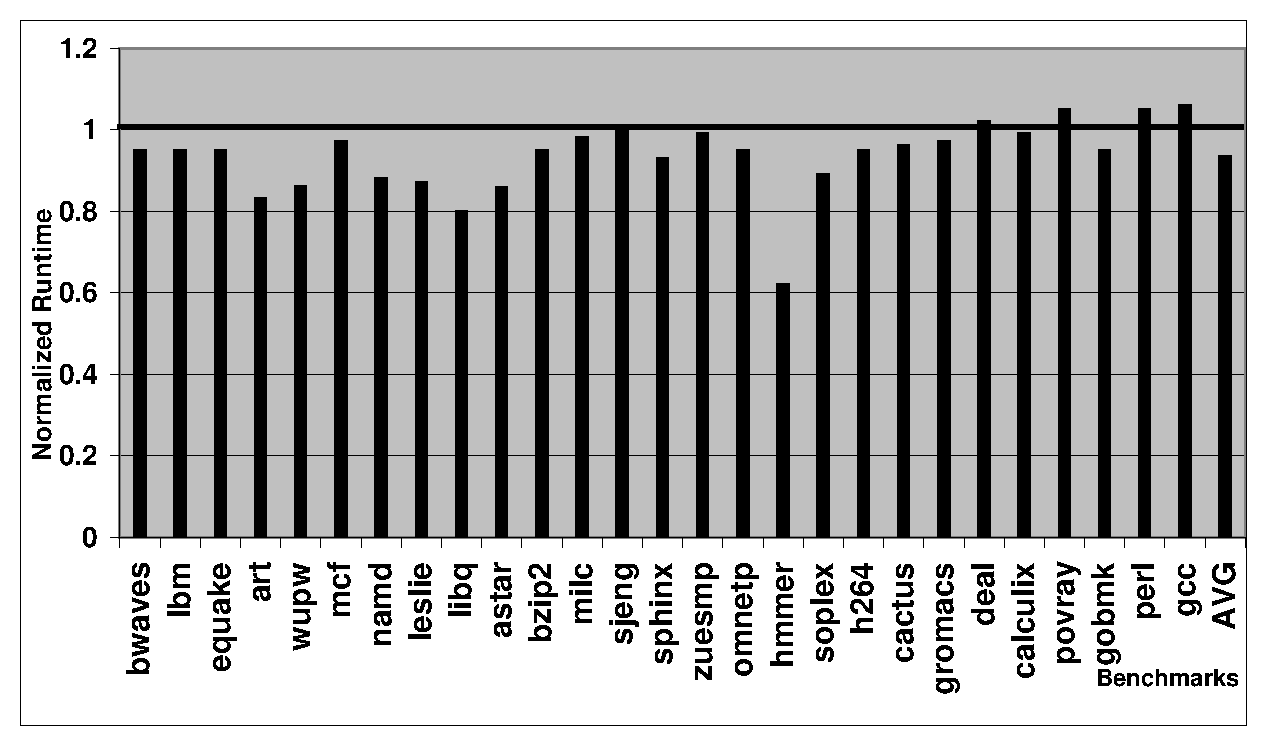
\includegraphics[width=\linewidth]{figures/EPS/optperf.eps}
\begin{scriptsize}
\caption{{{\textit{Normalized runtime of rewritten binary as compared to optimized gcc input binary (=1.0)}}}}
\label{fig:optimized}
\end{scriptsize}
}
\end{minipage} 
\hfill
\begin{minipage}{.28\linewidth}
\centering
{
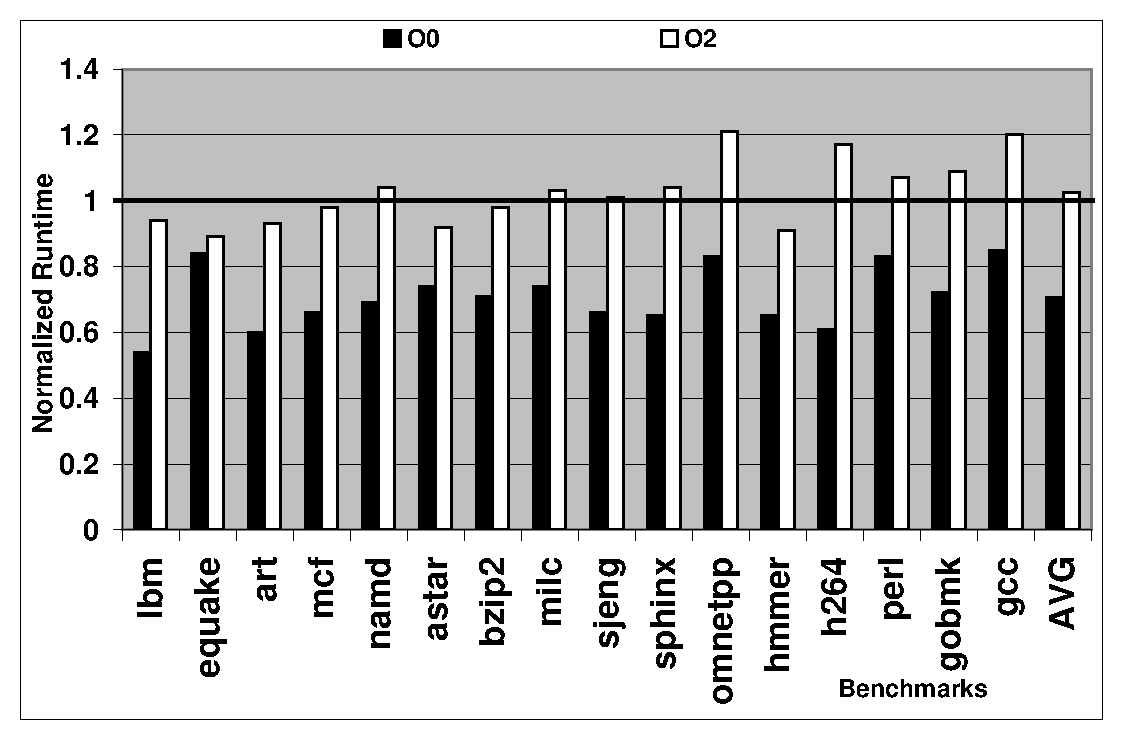
\includegraphics[width=\linewidth]{figures/EPS/pe-binaries.eps}
\begin{scriptsize}
\caption{{{\textit{Normalized runtime of rewritten binary as compared to its corresponding input version (=1.0) compiled by visual studio}}}}
\label{fig:visual-studio}
\end{scriptsize}
}
\end{minipage} 
\end{scriptsize}
}
\vspace{-3ex}
\end{figure*}



Fig~\ref{fig:OrigSymPromResult} relates the above promoted symbolic references to the original source-level artifacts. We enumerated the symbolic references in the input program using debug information (employed only for counting the references) and compared how many of these symbolic references are restored in the IR and the source code. It shows that our techniques are able to restore 66\% of the original symbolic references.

Fig~\ref{fig:PartResult} presents an insightful result regarding our partition algorithm (Alg~\ref{fig:algpartition}). On average, around 76\% of the memory locations have one partition, 18\% have two to five, and 6\% have five or more partitions. This is not unexpected since large procedures are relatively rare.

%the functioning of 
%
\begin{figure}[t]
{
%\vspace{-1in}
\centering
{
\begin{scriptsize}
\begin{tabular}{|c|c|c|c|} %|r|r|r|}
%xxxxx\=xxxxxxxxxxxxx\=xxxxxx\=xxxxxxxxxxx\=xxxxxx\=  \kill\\
\hline
\textbf{Program}&{\textbf{Version}}&{\textbf{Physical stack}}&{\textbf{Run Time Check}}\\ \hline
gcc&gcc-O0,VS-O0&117&0\\\hline
gcc&gcc-O3, VS-Ox&117&10\\	\hline
tonto&gcc-O0, gccO3&20&0\\	\hline
\end{tabular}
\caption {\scriptsize{\textit{Programs demonstrating corner cases of our analysis }}}
\label{fig:resultsCornerCases}
\end{scriptsize}
\vspace{-4ex}
}
}
\end{figure}

Fig~\ref{fig:resultsCornerCases} lists the programs which hit corner cases during the deconstruction of physical stack. The analysis of the original source code revealed that a physical stack frame was required for procedures that call \emph{alloca()}. Runtime checks are inserted in some procedures which accept a variable number of arguments using the \emph{va-arg} mechanism. Most of the procedures using \emph{va-arg} do not require runtime checks. This result establishes our earlier hypothesis that scenarios requiring run-time checks are extremely rare and consequently, have negligible overhead. Nonetheless, not handling these scenarios prohibits obtaining a functional IR and hence, are imperative for any translation system.

%\vspace{-3ex}
\subsection{Un-optimized input binaries}
Fig~\ref{fig:unoptimized} shows the normalized run-time of each rewritten binary compared to an input binary produced using gcc with no optimization (-O0 flag). Fig~\ref{fig:visual-studio} shows the corresponding run-time for binaries produced using Visual Studio compiler with no optimization (-O0 flag). We obtain an average improvement of 40\% in execution time for binaries produced by gcc and 30\% for binaries produced by Visual Studio, with an improvement of over 65\% in some cases (\emph{bwaves}). In fact, our tool brings down the normalized runtime of unoptimized input binaries from 2.2 to close to the runtime (1.25) of gcc-optimized binaries. (Graph not shown due to lack of space)
%his result shows that our rewriter is very useful for binaries that are not highly optimized.
%, such as legacy binaries(Graph not shown due to lack of space) %Fig~\ref{fig:unopt-cmp} compares the run-time of un-optimized input binary and the corresponding rewritten binary with an optimized binary produced directly by gcc. or binaries from compilers that are inferior compared to the today's best available compilers. 
%
%\footnote{We started experimenting with visual-studio binaries only recently and have presented the results for all the binaries which have been rewritten correctly. The runtime results are presented for visual studio binaries to demonstrate that our schemes are not compiler-dependent. Detailed experimental results are presented for gcc-produced binaries} 
%In most cases, after rewriting we raised the performance close to that of an optimized binary produced directly by gcc, showing the effectiveness of our approach.
%\input{figures/unoptperf}


\begin{figure*}[t]
{
%\centering
\vspace{-0.33in}
{
%\begin{minipage}[t]{.31\linewidth}
%\centering
%{
%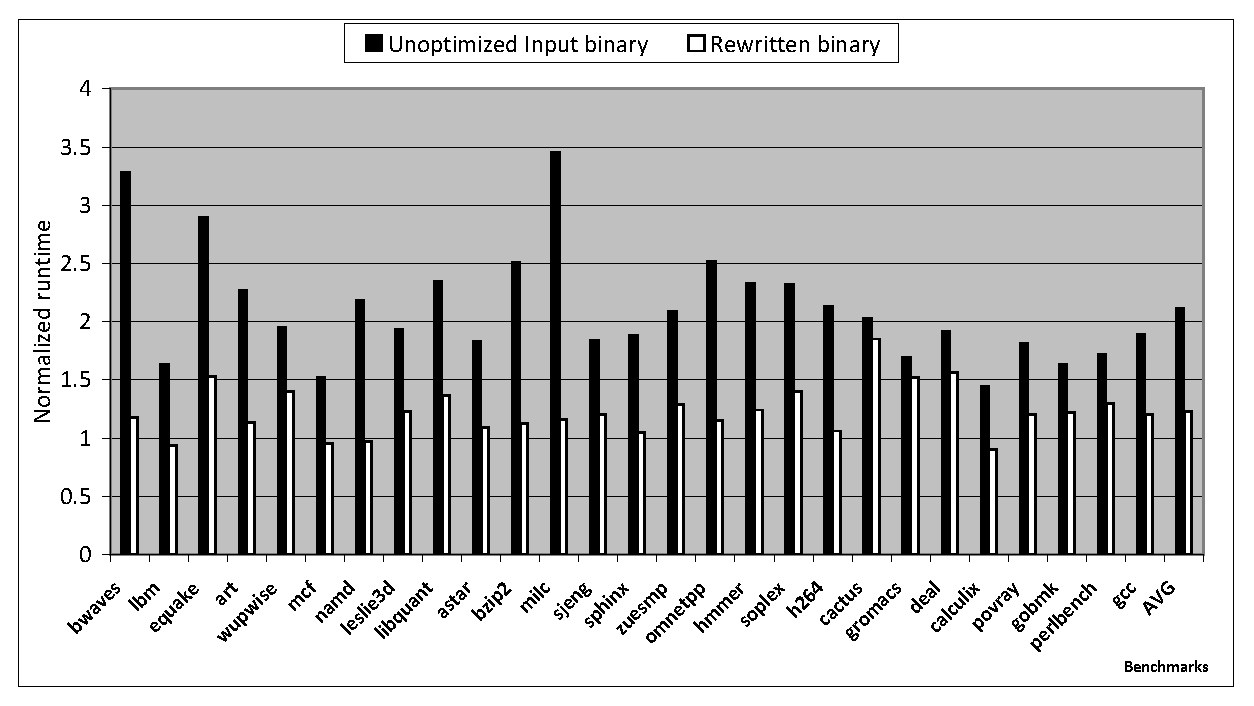
\includegraphics[width= 2.3 in]{figures/EPS/unopt-optcomp.eps}
%\caption{{\textit{Normalized runtime of unoptimized input binary and its rewritten version as compared to optimized input binary(=1.0)}}}
%\label{fig:unopt-cmp}
%}
%\end{minipage}
%\hfill
\begin{minipage}{.35\linewidth}
\centering
{
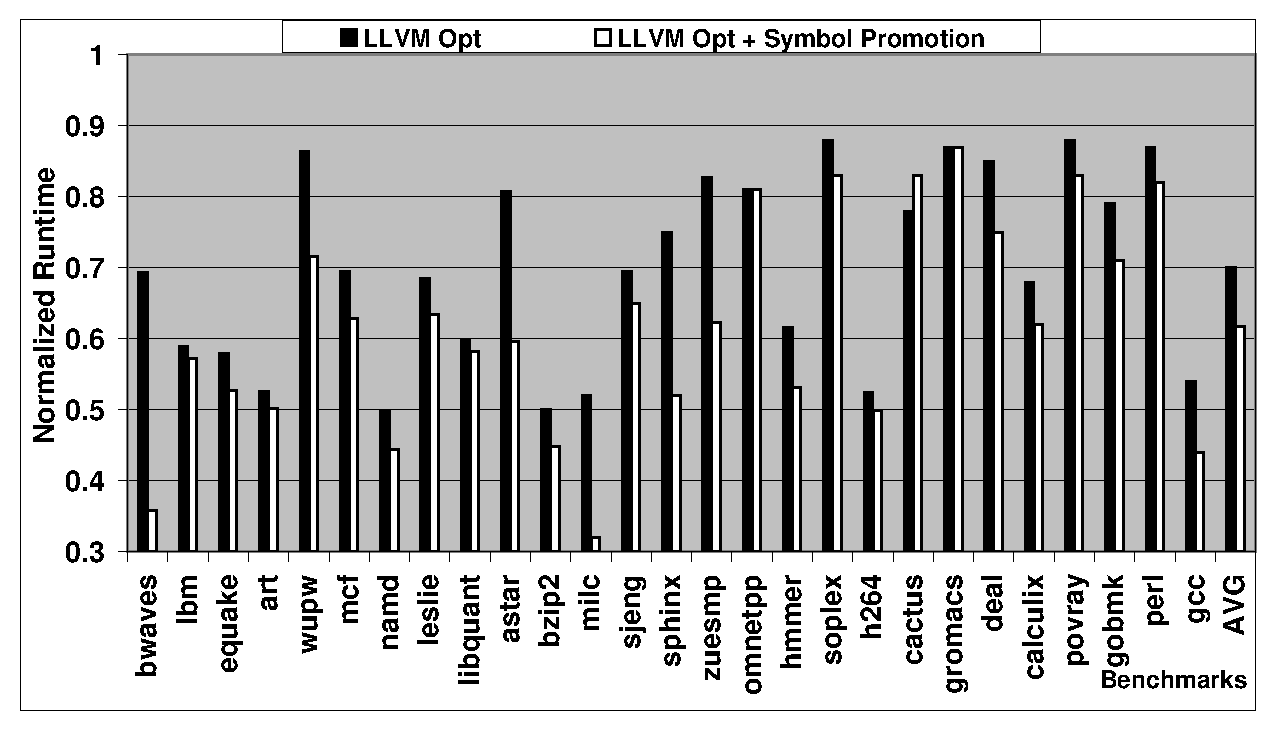
\includegraphics[width=\linewidth]{figures/EPS/impactunopt.eps}
\caption{{\textit{Impact of symbol promotion on runtime of rewritten binary v/s unoptimized input binary (=1.0) }}}
\label{fig:unopt-symprom}
}
\end{minipage}
\hfill 
\begin{minipage}{.35\linewidth}
\centering
{
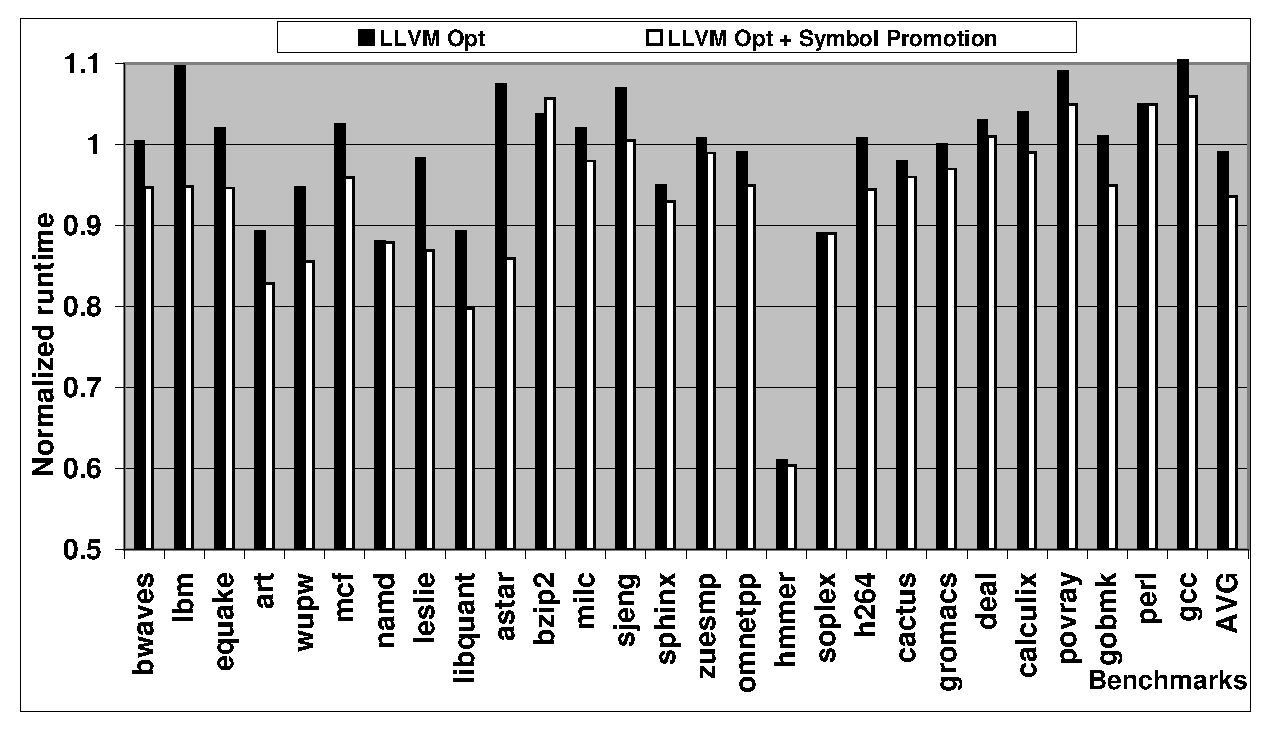
\includegraphics[width=\linewidth]{figures/EPS/impactopt.eps}
\caption{{\textit{Impact of symbol promotion on runtime of rewritten binary v/s optimized input binary (=1.0)}}}
\label{fig:opt-symprom}
}
\end{minipage}
\begin{minipage}{.29\linewidth}
\centering
{
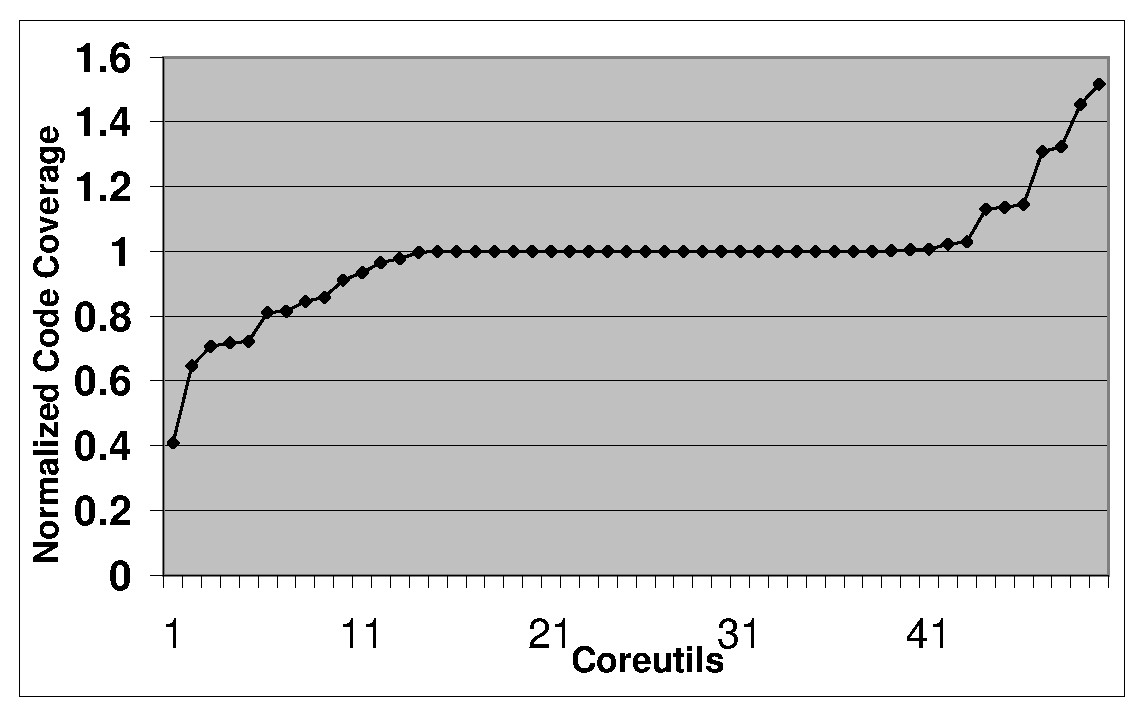
\includegraphics[width=\linewidth]{figures/EPS/klee-coverage.eps}
\caption{{\textit{Normalized code coverage in coreutils binaries as compared to source }}}
\label{fig:KleeCovRes}
}
\end{minipage}
}
\vspace{-4ex}
}
\end{figure*}


\begin{figure*}[t]
{
%\vspace{-0.2in}

%\centering
{
%\begin{minipage}[t]{.31\linewidth}
%\centering
%{
%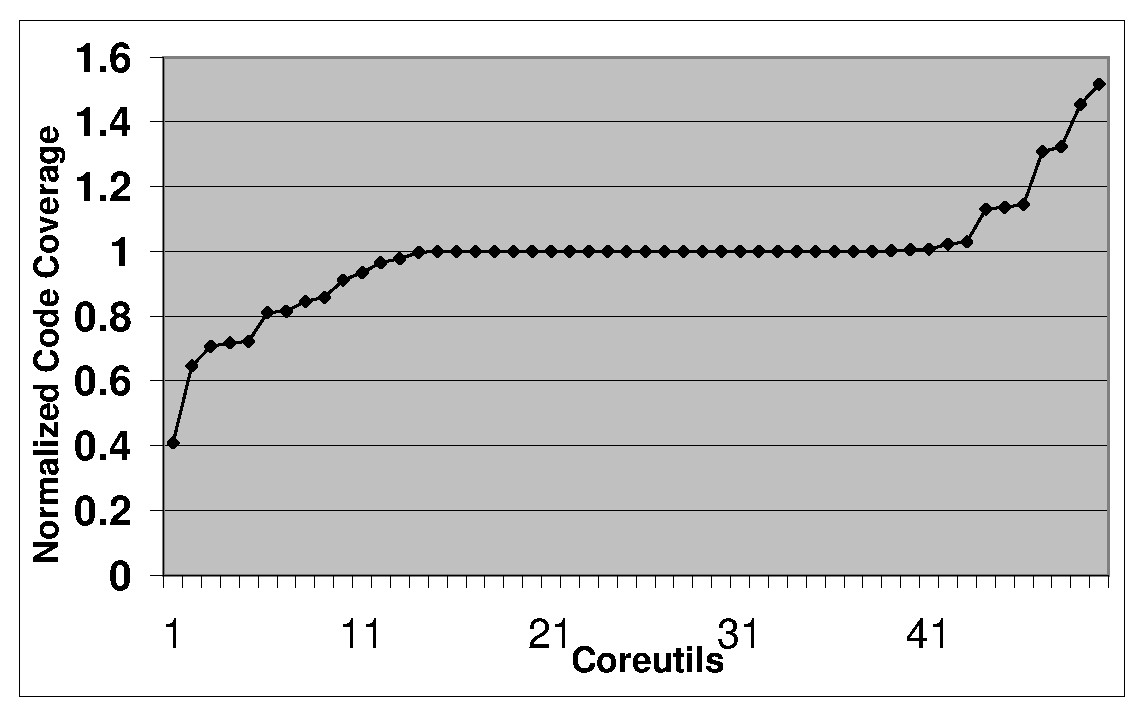
\includegraphics[width=2.1in]{figures/EPS/klee-coverage.eps}
%\caption{\scriptsize{\textit{Normalized code coverage in coreutils binaries as compared to source }}}
%\label{fig:KleeCovRes}
%}
%\end{minipage}

\begin{minipage}{.24\linewidth}
%\centering
{
\begin{scriptsize}
\begin{tabular}{|l|l|} %|r|r|r|}
%xxxxx\=xxxxxxxxxxxxx\=xxxxxx\=xxxxxxxxxxx\=xxxxxx\=  \kill\\
\hline
{mkdir -Z a b}&{mkdir -Z @@ -}\\ 
{mkfifo -Z a b}&{mkfifo -Z @@ -}\\ 
{mknod -Z a b p}&{mkdir -Z @@ - p@}\\ 
{seq -f \%0 1}&{seq -f \%1 1}\\ 
{paste -d\textbackslash \textbackslash   }&{paste -d\textbackslash \textbackslash   }\\ 
{\hspace{1ex}abcdefghijklmn}&{\hspace{1ex}@@@@@@@@ }\\ 
{}&{\hspace{1ex}@@@@@@ }\\  \hline
\end{tabular}
\caption {{\textit{Testcases for crashes (a)Source code~\cite{Cadar-KLEE} (b) Binaries }}}
\label{fig:result-symExec-testCases}
\end{scriptsize}%\vspace{-4ex}
}
\end{minipage}
%\begin{minipage}{.24\linewidth}
%\centering
%{
%\includegraphics[width=\linewidth]{figures/EPS/resultssymExecution-testCase.eps}
%\caption{{\textit{Test cases for crashes (a) Source code (b) Binaries}}}
%\label{fig:result-symExec-testCases}
%}
%\end{minipage}
\hfill
\hspace{1ex}
\begin{minipage}{.21\linewidth}
\centering
{
\begin{scriptsize}
\begin{tabular}{|l|l|l|} %|r|r|r|}
%xxxxx\=xxxxxxxxxxxxx\=xxxxxx\=xxxxxxxxxxx\=xxxxxx\=  \kill\\
\hline
{Binary}&{No}&{With}\\ 
{}&{Promotion}&{Promotion}\\ \hline
htget&980&4671\\ \hline
cut&1301&5103\\ \hline
split&1623&4104\\ \hline
\end{tabular}
\caption {{\textit{Improvement in constraints processing with symbol promotion }}}
\label{fig:results-symExecSymMem}
\end{scriptsize}%\vspace{-4ex}
}
\end{minipage}
\hfill
\hspace{1ex}
\begin{minipage}{.24\linewidth}
\centering
{
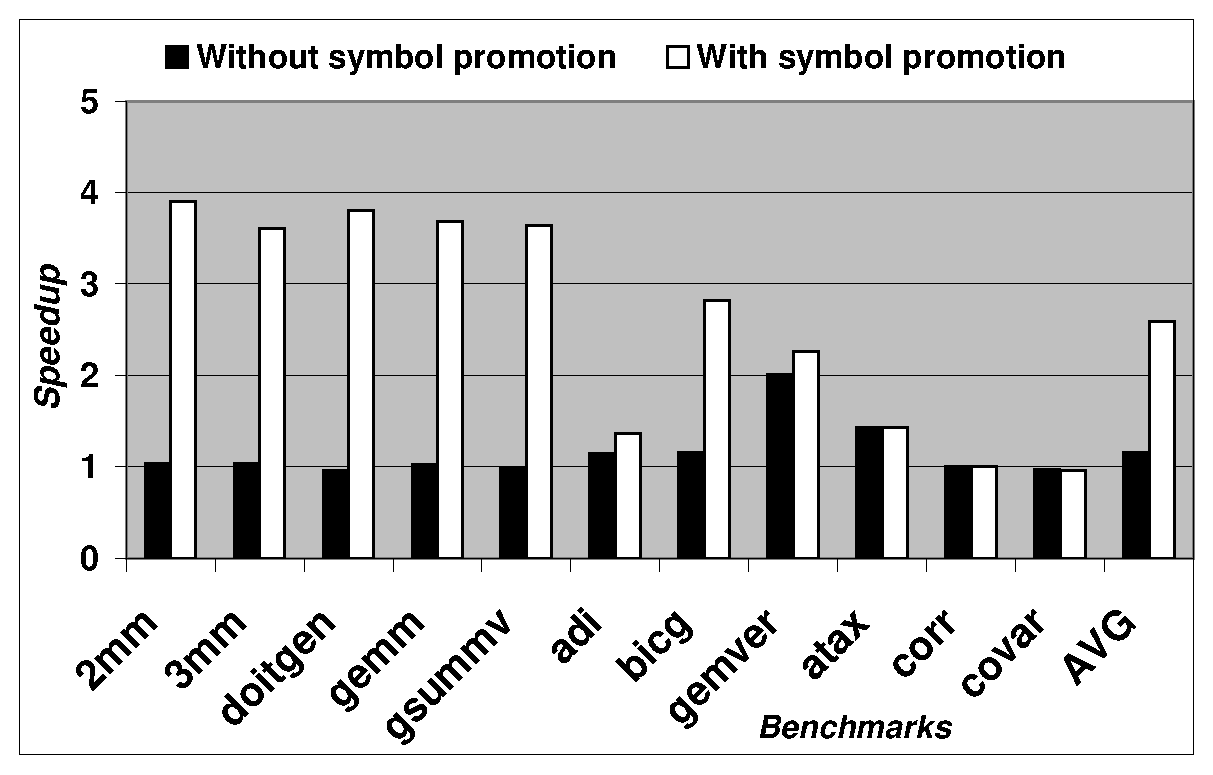
\includegraphics[width=\linewidth]{figures/EPS/parallel-runtime.eps}
\caption{{\textit{Automatic parallelization}}}
\label{fig:parallel-runtime}
}
\end{minipage} 
\hfill
%\hspace{-2ex}
\begin{minipage}{.24\linewidth}
\centering
{
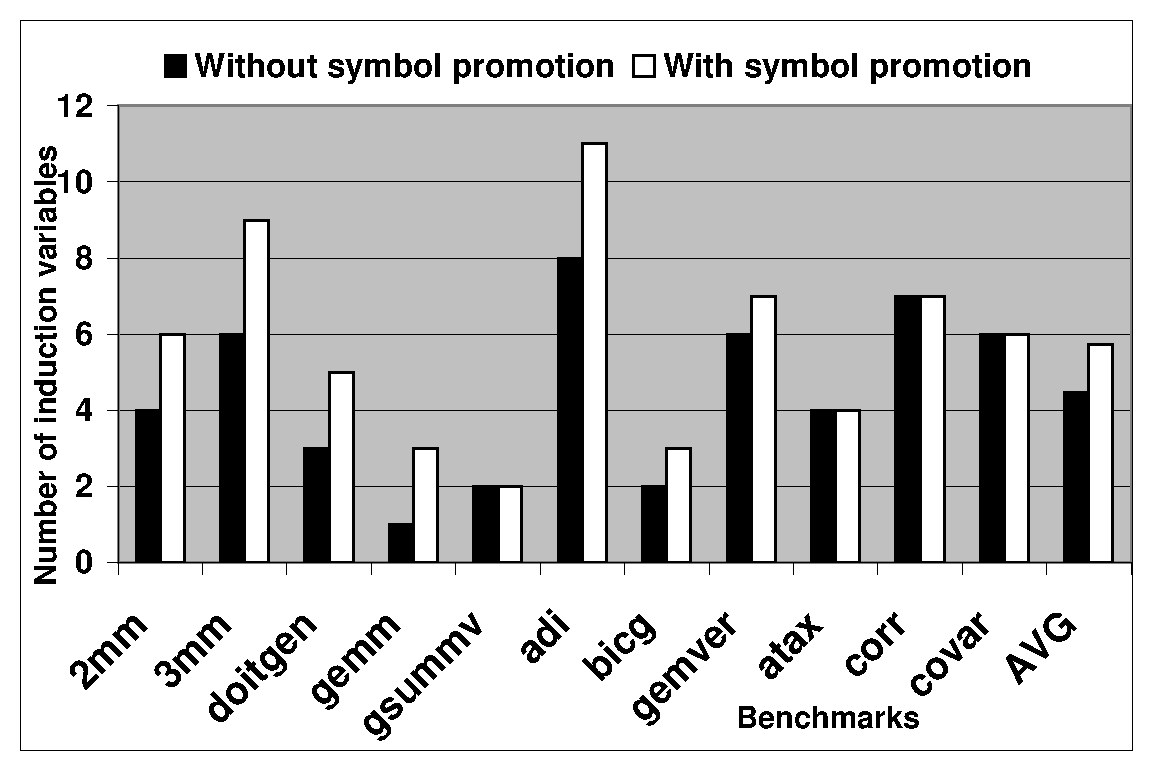
\includegraphics[width=\linewidth]{figures/EPS/induction-var.eps}
\caption{{\textit{Number of induction variables recognized}}}
\label{fig:parallel-indvar}
}
\end{minipage}
}
\vspace{-3ex}
}
\end{figure*}


\subsection{Optimized input binaries}
Fig~\ref{fig:optimized} shows the normalized execution time of each rewritten binary compared to an input binary produced using gcc with the highest-available level of optimization (-O3 flag). In this case, we obtain an average improvement of 6.5\% in execution time. It is interesting that we were able to obtain this improvement over already optimized binaries without any custom optimization of our own. One of our rewritten binaries (hmmer) had a 38\% speedup vs the input binary. Although GCC -O3 is known to produce good code, it missed the creation of few predicated instructions whereas LLVM did this optimization, explaining the speedup. Fig~\ref{fig:visual-studio} shows the corresponding run-time for binaries produced using Visual Studio compiler with full optimization flag (-O2). As evident, our framework was able to retain the performance of these binaries, with a small overhead of 2.7\% on average. 
%It exemplifies the underlying advantage of our binary rewriter - that it cumulates optimizations across two compilers -- rewritten binaries have an optimization if it is either present in the compiler that produced the input binary, or in the rewriter. This is why, for example, one of our rewritten binaries (hmmer) had a 38\% speedup vs the input binary. Although GCC -O3 is known to produce good code, it missed the creation of few predicated instructions whereas LLVM did this optimization, explaining the speedup. 
%In our case, if either GCC or LLVM had an optimization, the output binary should have it. , with one benchmark actually showing up a speedup of 38\% (hmmer)

%\input{figures/impact-symbol}
%\vspace{-2ex}
\subsection{Impact of symbol promotion}
Next, we substantiate the impact of symbol promotion on the run-time of rewritten binaries. Fig~\ref{fig:unopt-symprom} and Fig~\ref{fig:opt-symprom} show the normalized improvement in execution time obtained by applying only LLVM optimizations and by applying our symbol promotion techniques. It shows that symbol promotion is responsible for improving the average performance of rewritten binary from 30\% to 40\% in the case of unoptimized binaries (produced by gcc) and from 1\% to 6.5\% in the case of optimized binaries (produced by gcc). Since our cost metric is based on static profiling, we observed a small slowdown with symbol promotion in \emph{bzip2 O3}. 
%one of our benchmark 
%We reckon that symbol promotion accelerates the binaries in two ways: first, it serves as an implicit load-store forwarding optimization and secondly, it improves the efficiency of other optimizations. This result captures the combined effect of symbol promotion.

It is important to note that these results only measure the impact of symbol promotion. The impact of our method to convert physical frames to abstract frames is not measured above. However, we can infer that number since without obtaining abstract frames, none of the existing LLVM passes would run at all, leading to zero run-time improvement.	

%Fig~\ref{fig:static-impact} helps in quantifying the impact of symbol promotion on efficiency of individual compiler analysis. We chose three compiler analysis - copy propagation, constant propagation and dead-code elimination and collected their static performance statistics with and without the presence of symbols for three of our benchmarks. Fig~\ref{fig:static-impact} shows the normalized improvement in the number of static instances of each of these optimizations when using symbol promotion. Symbol promotion allows the compiler's copy propagation pass to implicitly implement store-load forwarding, explaining a large increase in copy propagation statistics. The effectiveness of other optimizations also improves considerably with the presence of symbols in the IR. 
 %hence the data for copy propagation has been scaled down by 10 to fit in the graph.

%Symbol promotion helps us in improving the quality of IR in general and makes it more suitable for analysis purposes. We analyze this subjective improvement by showing its impact on the C code obtained by compiler backend for ease of understanding. Fig~\ref{} shows an original C code and C code obtained from the binary with and without symbol promotion. As evident from this figure, the C code obtained after doing symbol promotion is more closer to the original source code. Having such detailed representation in C code would improve the existing analysis frameworks for binaries with no source code e.g. legacy binaries.

\subsection{Symbolic Execution}

%%\begin{figure}[t]
%\vspace{-0.5in}
%\centering
%\psfig{figure=figures/plots/runtimeFinal.eps,width=5.5in} }
%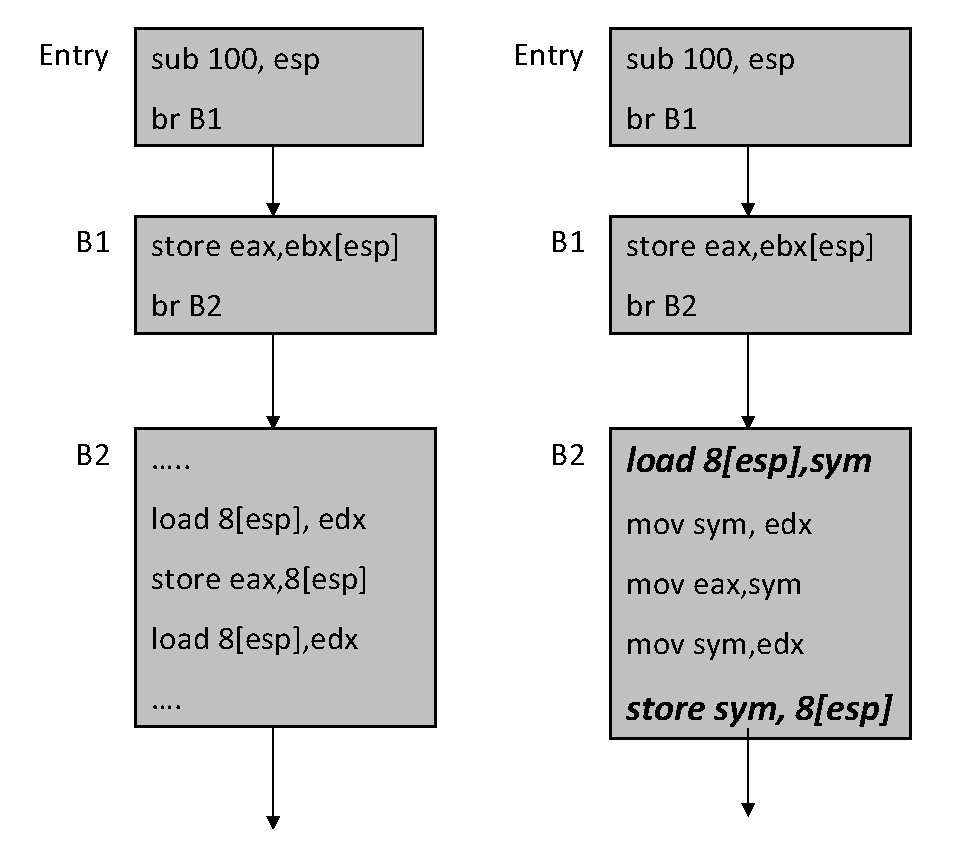
\includegraphics [width=0.5\linewidth] {figures/EPS/cfgex.eps} 
%\tiny{
%\caption { \textit{Stack layout in a binary}}
%}
%\label{fig:stack-layout}
%\end{figure}

\begin{figure}[b]
{
\vspace{-2ex}
\centering
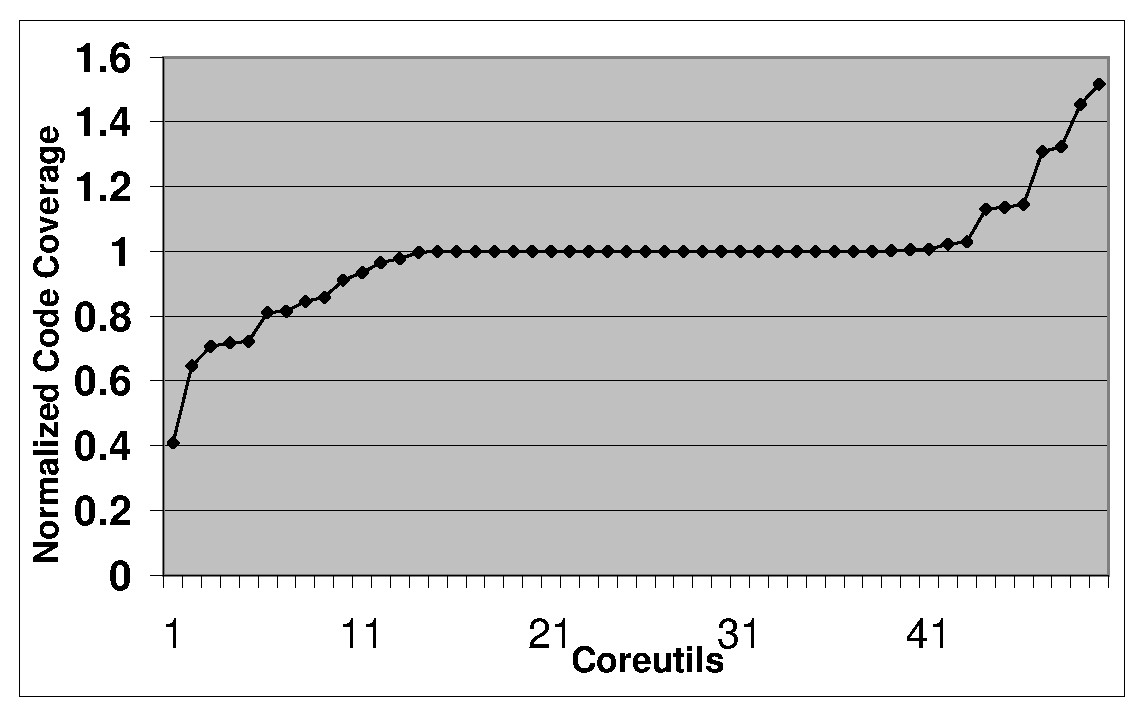
\includegraphics[width=0.6\linewidth]{figures/EPS/klee-coverage.eps}
\caption{\textit{Normalized code coverage in coreutils binaries as compared to source }}
\label{fig:KleeCovRes}
}
%\hfill
\vspace{-5ex}
\end{figure}




%\begin{figure}[t]
%{
%\centering
%\begin{minipage}{.6\linewidth}
%{
%\centering
%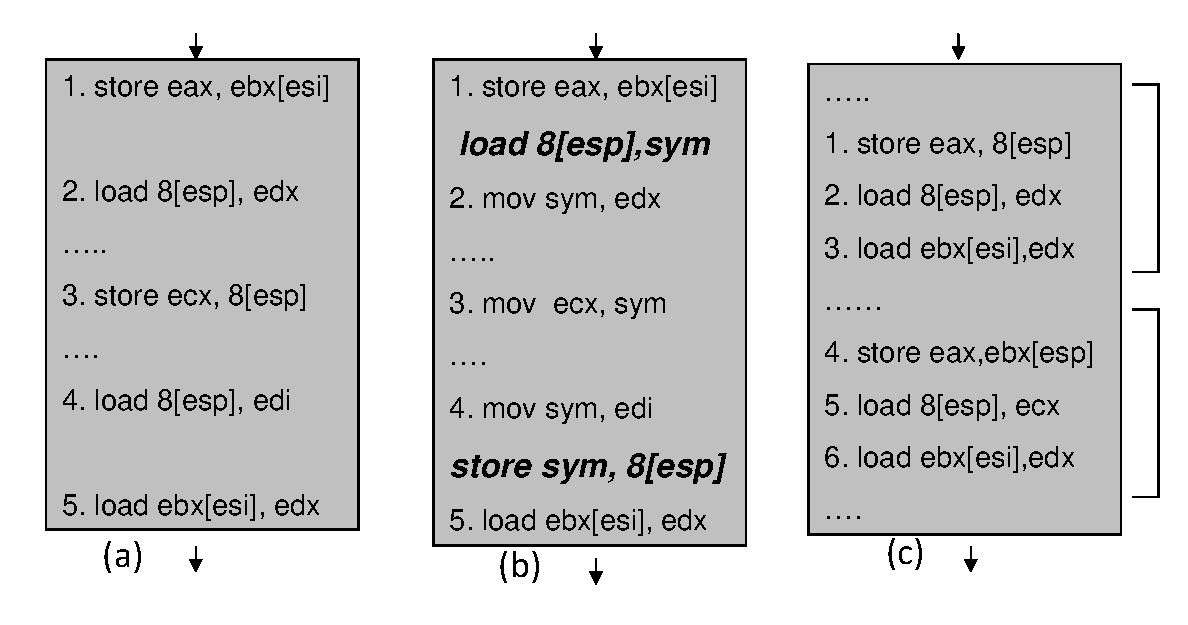
\includegraphics[width=0.5\linewidth]{figures/EPS/pathcfg.eps}
%\caption{\textit{Path dependent promotion. Second operand in the instruction is the destination of the instruction. }}
%\label{fig:PromExample}
%}
%\vspace{-0.1in}
%\end{minipage}
%%\hfill
%\begin{minipage}{0.3\linewidth}
%{
%\centering
%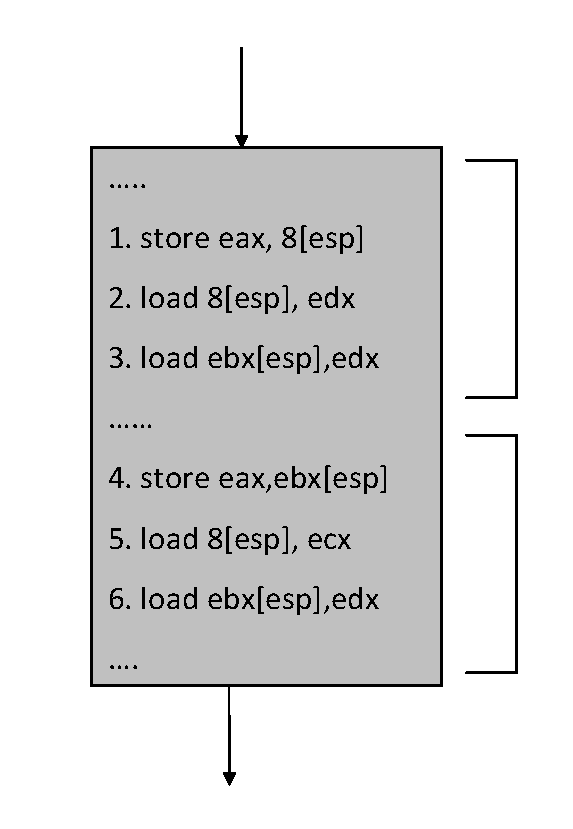
\includegraphics[width=0.3\linewidth]{figures/EPS/partitioncfg.eps} 
%\caption{\textit{Motivation for partition}}
%\label{fig:PartExample}
%}
%\vspace{-0.1in}
%\end{minipage}
%}
%\vspace{-0.2in}
%\end{figure}

%Code coverage
KLEE is efficiently designed to obtain a high code coverage on source programs. We run KLEE in our framework on a set of 50 coreutils binaries and compare the resulting code coverage with that achieved by KLEE on the corresponding source code in Fig~\ref{fig:KleeCovRes}. Our framework achieves a code coverage of 73\% on average compared to 76\% obtained by KLEE on source programs. 
%This experiment demonstrates that symbolic execution using KLEE on the IR produced by our framework achieves almost similar coverage as it achieves on source code.

%\begin{figure}[t]
{
%\vspace{-1in}
\centering
\includegraphics[width=0.5\linewidth]{figures/EPS/resultssymExecution-testCase.eps}
\vspace{-3ex}
\caption{\textit{KLEE generated test cases for crashes in coreutils (a) Source code (as reported by KLEE paper) (b) Binaries (Generted in our framework)}}
\label{fig:result-symExec-testCases}
}
\vspace{-4ex}
\end{figure}

%bug detection
KLEE has been shown to detect various bugs in a particular version of coreutils (6.10). Fig~\ref{fig:result-symExec-testCases} lists the test cases generated through our framework and those reported in the original KLEE paper\footnote{The original KLEE paper shows 10 bugs in coreutils but latest version of KLEE only detects five of these bugs}. Note that the original KLEE paper detected these bugs from source code, but our framework detected the same bugs from binaries. Both these results demonstrate the unique ability of our framework to efficiently employ source level research directly for executables. 
%This shows that our framework is able to reliably detect the bugs which are detected by directly applying symbolic execution of source code., and generate corresponding test cases for each detected bug,

%\begin{figure}[t]
{
\begin{minipage}[t]{.4\linewidth}
\centering
{
\begin{scriptsize}
\begin{tabular}{|c|c|c|} %|r|r|r|}
%xxxxx\=xxxxxxxxxxxxx\=xxxxxx\=xxxxxxxxxxx\=xxxxxx\=  \kill\\
\hline
{Binary}&{No}&{With}\\ 
{}&{Promotion}&{Promotion}\\ \hline
htget&980&4671\\ \hline
cut&1301&5103\\ \hline
split&1623&4104\\ \hline
\end{tabular}
\caption {\scriptsize{\textit{Improvement in constraints processing with symbol promotion }}}
\label{fig:results-symExecSymMem}
\end{scriptsize}%\vspace{-4ex}
}
\end{minipage}
\hfill
\begin{minipage}[t]{.5\linewidth}
\centering
{
\includegraphics[width=\linewidth]{figures/EPS/resultssymExecution-testCase.eps}
\caption{\scriptsize{\textit{Test cases for crashes in coreutils (a) Source code (KLEE paper) (b) Binaries (Our framework)}}}
\label{fig:result-symExec-testCases}
}
\end{minipage}
}
\vspace{-4ex}
\end{figure}

%symbolic memory
Recall from Sec~\ref{sec:symExec}, symbol promotion enables our framework to efficiently reason about symbolic memory accesses. We run symbolic execution on IR produced from binaries for 30 minutes and compare the result in two scenarios: with and without symbol promotion. Fig~\ref{fig:results-symExecSymMem} shows that the presence of symbol promotion greatly improves the number of constraints processed by the solver, resulting in a much higher code coverage in the same amount of time. Program \emph{htget} has been shown to have a bug~\cite{Brumley-Mayhem} and we were able to detect that bug within 5 minutes in the presence of symbols as opposed to 25 minutes without symbol promotion.
%\footnote{KLEE simulates symbolic memory for only concrete-size memory objects, hence, variable-sized memory allocations in the above programs had to be replaced by fixed size allocations.}
%bug fix

Further, the presence of a rewriting path in our framework enables us to remedy the above detected bugs in binaries. We analyzed the dump for one of the coreutil binary (\emph{mkdir}), fixed the corresponding behavior in IR and obtained a rewritten bug-free binary.
%    us application synergizing the symbolic execution and rewriting path of our framework. As evident from Fig~\ref{fig:result-symExec-testCases}, KLEE detects a bug in mkdir coreutil binary. Analysis of the dump revealed that the error arises when an invalid global location is passed to a print function. We were able to fix this behaviour in IR and obtained a rewritten binary which didn't display this bug.

%Next, we demonstrate an interesting application synergizing the symbolic execution and rewriting path of our framework. As evident from Fig~\ref{fig:result-symExec-testCases}, KLEE detects a bug in mkdir coreutil binary. Analysis of the dump revealed that the error arises when an invalid global location is passed to a print function. We were able to fix this behaviour in IR and obtained a rewritten binary which didn't display this bug.

%Fig~\ref{} shows the corresponding dump in case of mkdir coreutil. 
%The original KLEE framework dumps the location of each detected bug in the input source code. Since a standalone binary does not contain debug information, we modified KLEE to dump the corresponding buggy location in LLVM IR. In fact, the original error as reported by KLEE in mkdir is related to \emph{optarg} being passed as emph{NULL}.

\subsection{Automatic Parallelization}
Kotha et al~\cite{micro-aparna10} presented a method for automatic parallelization for binaries. Here, we substantiate the impact of symbol promotion on their methods for a subset of \emph{PolyBench} and \emph{Stream} suite. Fig~\ref{fig:parallel-runtime} shows that symbol promotion increases the speedup by 2.25x for 4 threads.
%of 11 benchmarks

The underlying reason for the speedup is that symbol promotion enables discovery of more induction variables. Many induction variables for outer loops are often present on the stack instead of registers. Consequently, such induction variables are not detected by compiler methods, resulting in parallelization of inner loops, which have high synchronization overhead. As shown in Fig~\ref{fig:parallel-indvar}, symbol promotion enables the discovery of more induction variables, enabling the parallelization of more beneficial outer loops.

%We further investigate why symbol promotion helped automatic parallelization significantly. In order to parallelize loops using an affine automatic parallelizer, it is essential to recognize induction variables. We observe that for x86 binaries, many induction variables, for affine loops of nesting depth greater than two, are often present on the stack instead of registers;  the compiler's induction variable recognizer based on symbols fails to recognize them. This results in parallelization of only inner loops even though outer-loop parallelization is legal. Parallelizing inner loops involves a significant synchronization overhead resulting in a lower speedup. On the other hand, symbol promotion promotes the stack allocated-induction variables corresponding to outer loops also to symbols; consequently, these induction variables get recognized and it allows the parallelizer to do parallelization on more beneficial outer loops. Fig~\ref{fig:parallel-indvar} shows the number of outer loops for which induction variables are recognized with and without symbol promotion.
%Further, for affine loops of nesting depth greater than two, induction variables of outer loops are generally placed on the stack. 

%hence we parallelize inner loops when symbol promotion is not performed even though outer-loop parallelization is legal
%In affine loops of nesting depth greater than two, induction variables of outer loops are generally placed on the stack since there are no free registers for them. To parallelize these loops using the most basic affine automatic parallelizer on binaries, it is essential to recognize these locations on stack and promote them to variables, which will enable the compiler's induction variable recognizer to recognize them as induction variables. We observe that for x86 binaries compiled using gcc -O3 many induction variables are often present on the stack and hence we parallelize inner loops when symbol promotion is not performed even though outer-loop parallelization is legal. Parallelizing inner loops implies that there is a significant overhead due to synchronization and hence the speedup is lower than the case when symbol promotion is performed. A detailed statistics of number of outer loops for which induction variables recognized with and without symbol promotion is presented in figure~\ref{fig:parallel-indvar}. 

%We conclude by associating the advantages of a compiler IR based rewriter listed in ~\ref{sec:intro} with our results. Automatic parallelization and security enforcements depict that compiler IR allows any complex code transformation in a rewriter as well as ability to reuse compiler research methods. Further, the application of existing LLVM compiler analysis depict the reuse of compiler passes. The improvement in induction variable recognition and alias analysis show that the compiler analysis perform better with presence of symbols. Also, the better quality of C code show that presence of symbols make IR more favorable to analysis. In future work, we would 